\documentclass[12pt,a4paper]{article} 
\usepackage[portuguese]{babel} \usepackage[utf8]{inputenc}
\usepackage{amsmath} 
\usepackage{graphicx}
\usepackage{booktabs}
\usepackage{float}
\begin{document}
\setcounter{figure}{2}
\setcounter{section}{3}
\setcounter{page}{4}
\section{Relatório}
\subsection{Introdução}

Nesta prática, deseja-se entender o funcionamento de um circuito integrado temporizador \emph{LM555}, e suas aplicações como um multivibrador monoestável e como um multivibrador astável (cirucito oscilador). 

Um vibrador monoestável é um circuito eletrônico que gera um pulso de saída. Quando desencadeado, um pulso de duração pré-defnida é produzido.
O circuito então retorna para seu estado de repouso e não produz outro sinal de saída até ser desencadeado novamente.

Um multivibrador é um circuito eletrônico usado para implementar uma variedade de dispositivos simples de dois estados como osciladores de relaxação, timers e flip-flops.
Ele consiste de dois dispositivos amplificadores (transistores, tubos de vácuo ou outros dispositivos) acoplado com resistores e capacitores.
O primeiro circuito multivibrador, o circuito multivibrador astável, foi inventado por Henri Abraham e Eugene Bloch durante a primeira guerra mundial. 
Eles chamaram de circuito multivibrador pois a forma de onda da saída era rica em harmônicos. 
Já um multivibrador astável é um circuito que não está estável em nenhum estado; continuamente troca de um estado para outro. Este funciona como oscilador de relaxação.

No experimento, o circuito integrado LM555 foi escolhido pois ele pode operar tanto como em uma configuração monoestável e astável. O diagrama descrito pela Figura~\ref{fig:0} evidencia que função cada pino exerce.

\begin{figure}[htpb]
  \centering
  \includegraphics[width=0.8\linewidth]{name.ext}
  \caption{Name}
  \label{fig:name}
\end{figure}
\subsection{Análises}
No experimento 1, escolhemos os valores de resistência  e capacitância adequado a fim de obter um pulso de duração previamente escolhida, no caso $1ms$. Os valores foram de $R=100k \Omega$ e $500 pF$ (obtido através de dois capacitores de $1 nF$ em série). Estes valores foram escolhidos através do datasheet e validados através da montagem do circuito.   O resultado se encontra na Figura~\ref{fig:1}
\begin{figure}[htpb]
  \centering
  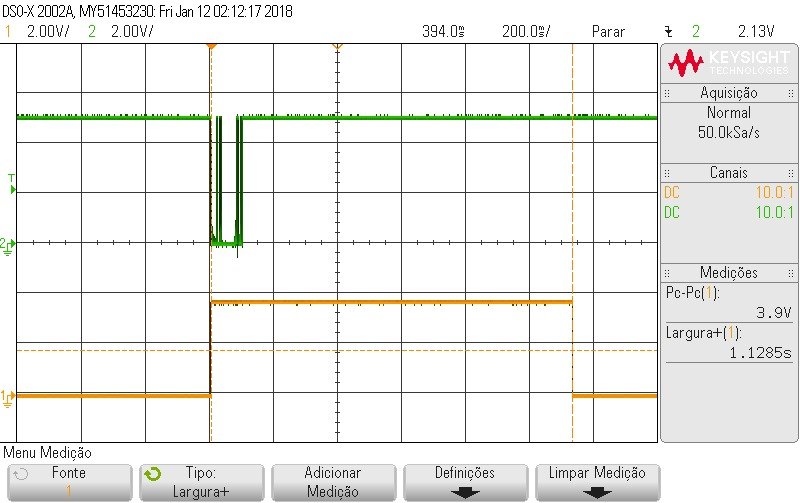
\includegraphics[width=0.8\linewidth]{img/exp1.jpg}
  \caption{Saída do circuito multivibrador monoestável descrito pela Figura~1.}
  \label{fig:1}
\end{figure}

No experimento 2, montou-se o circuito descrito na Figura~2 e com o potenciômetro configurado com seu valor mínimo e seu valo máximo foram obtidos os gráficos das Figuras~\ref{fig:2}-\ref{fig:3}.
\begin{figure}[htpb]
  \centering
  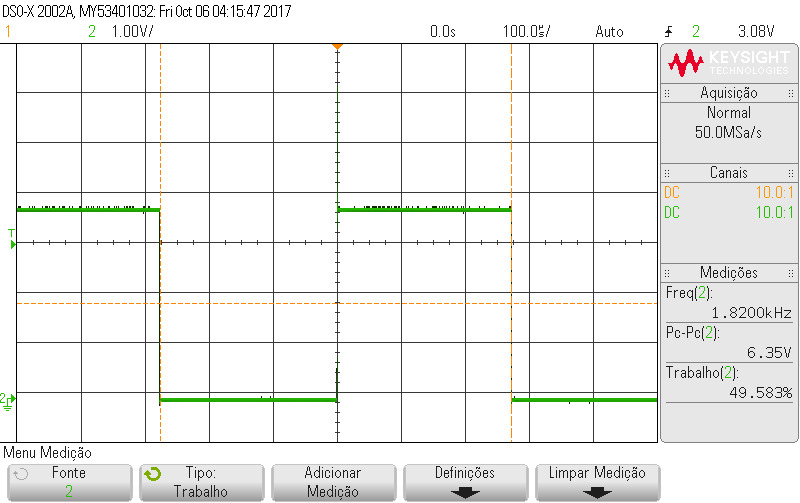
\includegraphics[width=0.8\linewidth]{img/min.jpg}
  \caption{Saída do circuito oscilador descrito na Figura~2, com o potenciômetro em seu valor mínimo. }
  \label{fig:2}
\end{figure}

\begin{figure}[htpb]
  \centering
  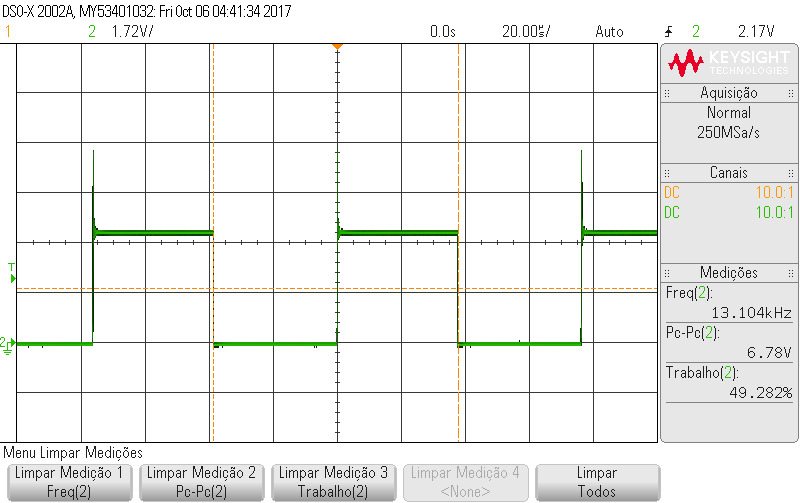
\includegraphics[width=0.8\linewidth]{img/max.jpg}
  \caption{Saída do circuito oscilador descrito na Figura~2, com o potenciômetro em seu valor máximo. }
  \label{fig:3}
\end{figure}
\subsection{Discussoes}
No circuito da Figura~1 o circuito integrado LM555 age como um timer que gera um pulso. Este pulso começa quando o LM555 recebe um sinal na pinagem do trigger que caí abaixo de $1/3$ da tensão da fonte de alimentação. A largura do pulso de saída é determinado pela constante de tempo da rede $RC$. O pulso termina quando o capacitor se igual a $2/3$ da tensão de alimentação. Este pulso de saída pode ser extendido ou diminuído dependendo de cada aplicação ajustando os valores de $R$ e $C$. 
\subsection{Conclusão}
\end{document}
